%************************************************
\chapter{Assessment of current Business Process Management Solutions}\label{ch:assessment}
%************************************************

The lack of flexibility in handling event subscription in business processes has been outlined in the previous chapters, and a set of additional requirements \textit{R1} to \textit{R3} for process management solutions have been presented.
In this section, we take a closer look at the capabilities of current solutions with regards to the event occurrence scenarios~(see~\autoref{ch:ps:eos}) to get a better understanding of the issues that arise when working with event subscription in business processes.

The assessment will be carried out on the basis of the \ac{BPMN} and Camunda, a state-of-the art and widely adopted business process engine~(\autoref{ch:bg:bpms}). Both tools shall be used \textit{as they are}, that means without utilizing their comprehensive extension mechanisms.
The main goal is to identify and illustrate the shortcomings of the current process technology stack by attempting to implement the requirements identified previously.
We therefor first investigate options to handle the \acs{EOS}s on the BPMN model level~(\autoref{ch:ass:models}) and then proceed to implementing early event subscription and event buffering in a set of Camunda processes~(\autoref{ch:assessment-implementation}).

Finally, the findings are discussed in \autoref{ch:ass:discussion} which leads to the presentation of three additional requirements, \textit{R4} to \textit{R6}.
The extended requirements will be referenced in \autoref{ch:flexibleeventsubscription} to develop a more refined subscription handling model.

\todo[inline]{which functionality should be evaluated exactly?: all requirements? all occurrence scenarios, but no buffer policies. The buffer will always store the last version of the event and also deliver that version.}


\section{BPMN Models in presence of the Event Occurrence Scenarios}\label{ch:ass:models}

According the BPMN specification, the listening for an event starts only when the event element is enabled. The start of the listening is interpreted as the time of event subscription.
The motivating examples illustrate that process executions can be delayed or even blocked because of a late time of event subscription~(\autoref{ch:motivatingexamples}).
The subscription-time is put in relation to the time of event occurrence by the help of the event occurrence scenarios.

In this section, I first describe for each \ac{EOS} how a basic event implementation behaves in presence of the given scenario.
I then evaluate if it is possible to create a BPMN model that is free from unnecessary delay in these situations.
The investigations are carried out on the basis of the abstract process model shown in \autoref{fig:abstract-process-with-event}.
It uses an intermediate message catch event which follows an arbitrary process flow, represented through a collapsed sub-process.
The process terminates after the event is received.
It is assumed, that the event can occur independently from the preceding subprocess and therefor in accordance with any of the event occurrence scenarios. That enables us to investigate each EOS using this simple model.
The event behavior is comparable with the \textit{Eurotunnel Delay Event} considered in \textit{Example~1.1}\,. Depending on the discussed EOS, the motivating examples will be used for further illustration of the situations.

\todo[inline]{this evaluates requirement 2}


\begin{figure}[]
	\myfloatalign
	{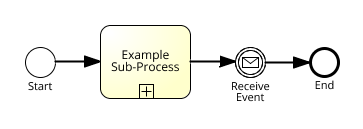
\includegraphics[width=0.7\linewidth]{chapters/assessment/generic-process-with-interm-event.png}}
	\caption{Generic process terminating after an intermediate message catch event}\label{fig:abstract-process-with-event}
\end{figure}


\subsection*{EOS1: The event occurs while the catch element is enabled}

The first scenario represents the case that is assumed by the BPMN 2.0 specification: 
The event occurs after the event element has been enabled and before it has terminated. It will be consumed by the catch event and the process flow can proceed without unnecessary delay.
In this scenario, the use of a simple intermediate catch event is sufficient.

Notably, there always is a certain delay when consuming an event through an intermediate catch event. The BPMN specification itself states that \textit{the handling consists of waiting for the Event to occur}.
However, that delay can theoretically be infinitely small. 
We speak of an \textit{unnecessary} delay in the context of flexible event subscription if an earlier subscription time would have meant a reduced waiting time for the event.

\subsection*{EOS2: The event does not occur}

\begin{figure}[bth]
	\myfloatalign
	\subfloat[Parallel timer event]
	{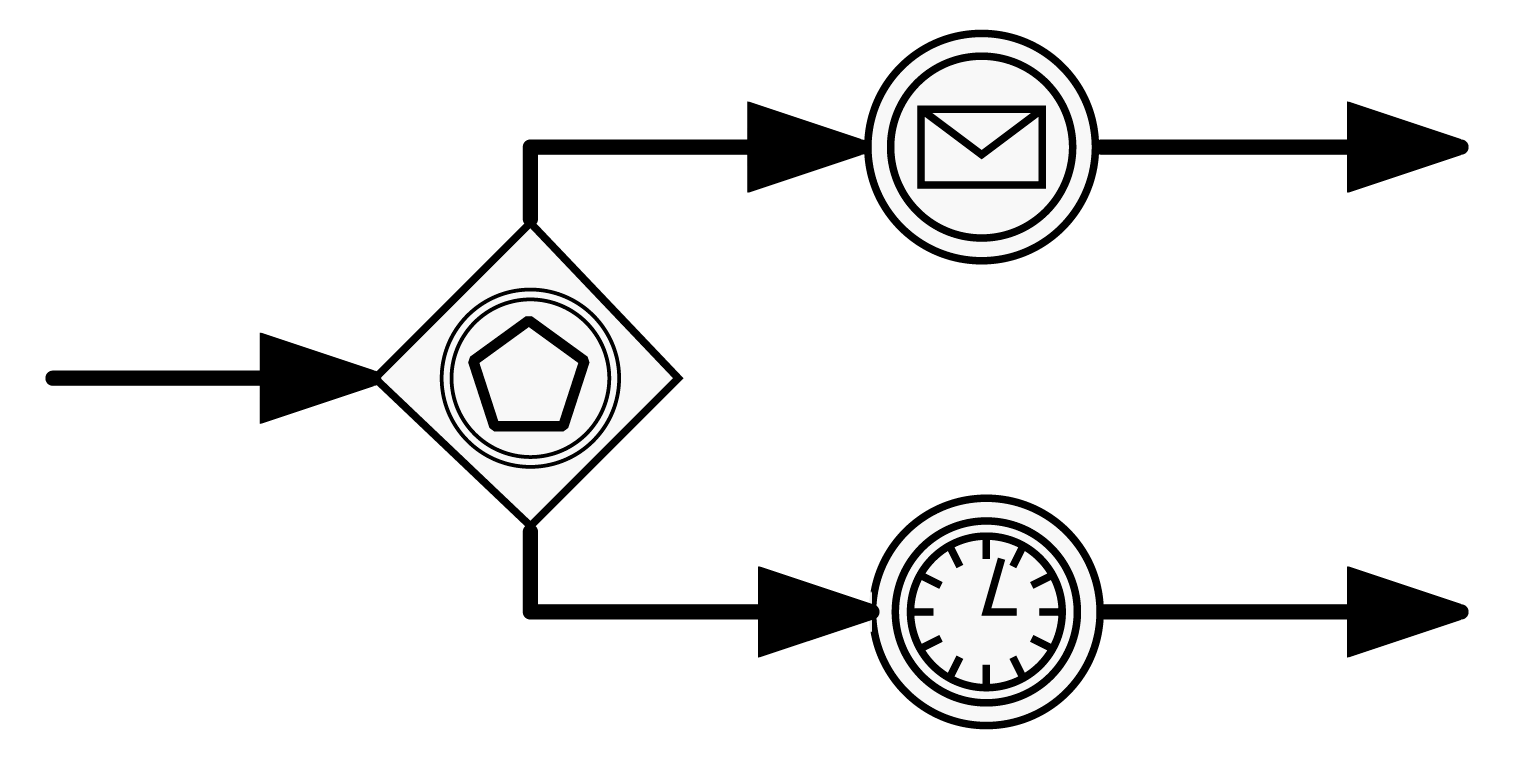
\includegraphics[width=.45\linewidth]{chapters/assessment/parallel-timer-event.png}} \quad
	\subfloat[Boundary timer event]
	{%\label{fig:example-b}%
		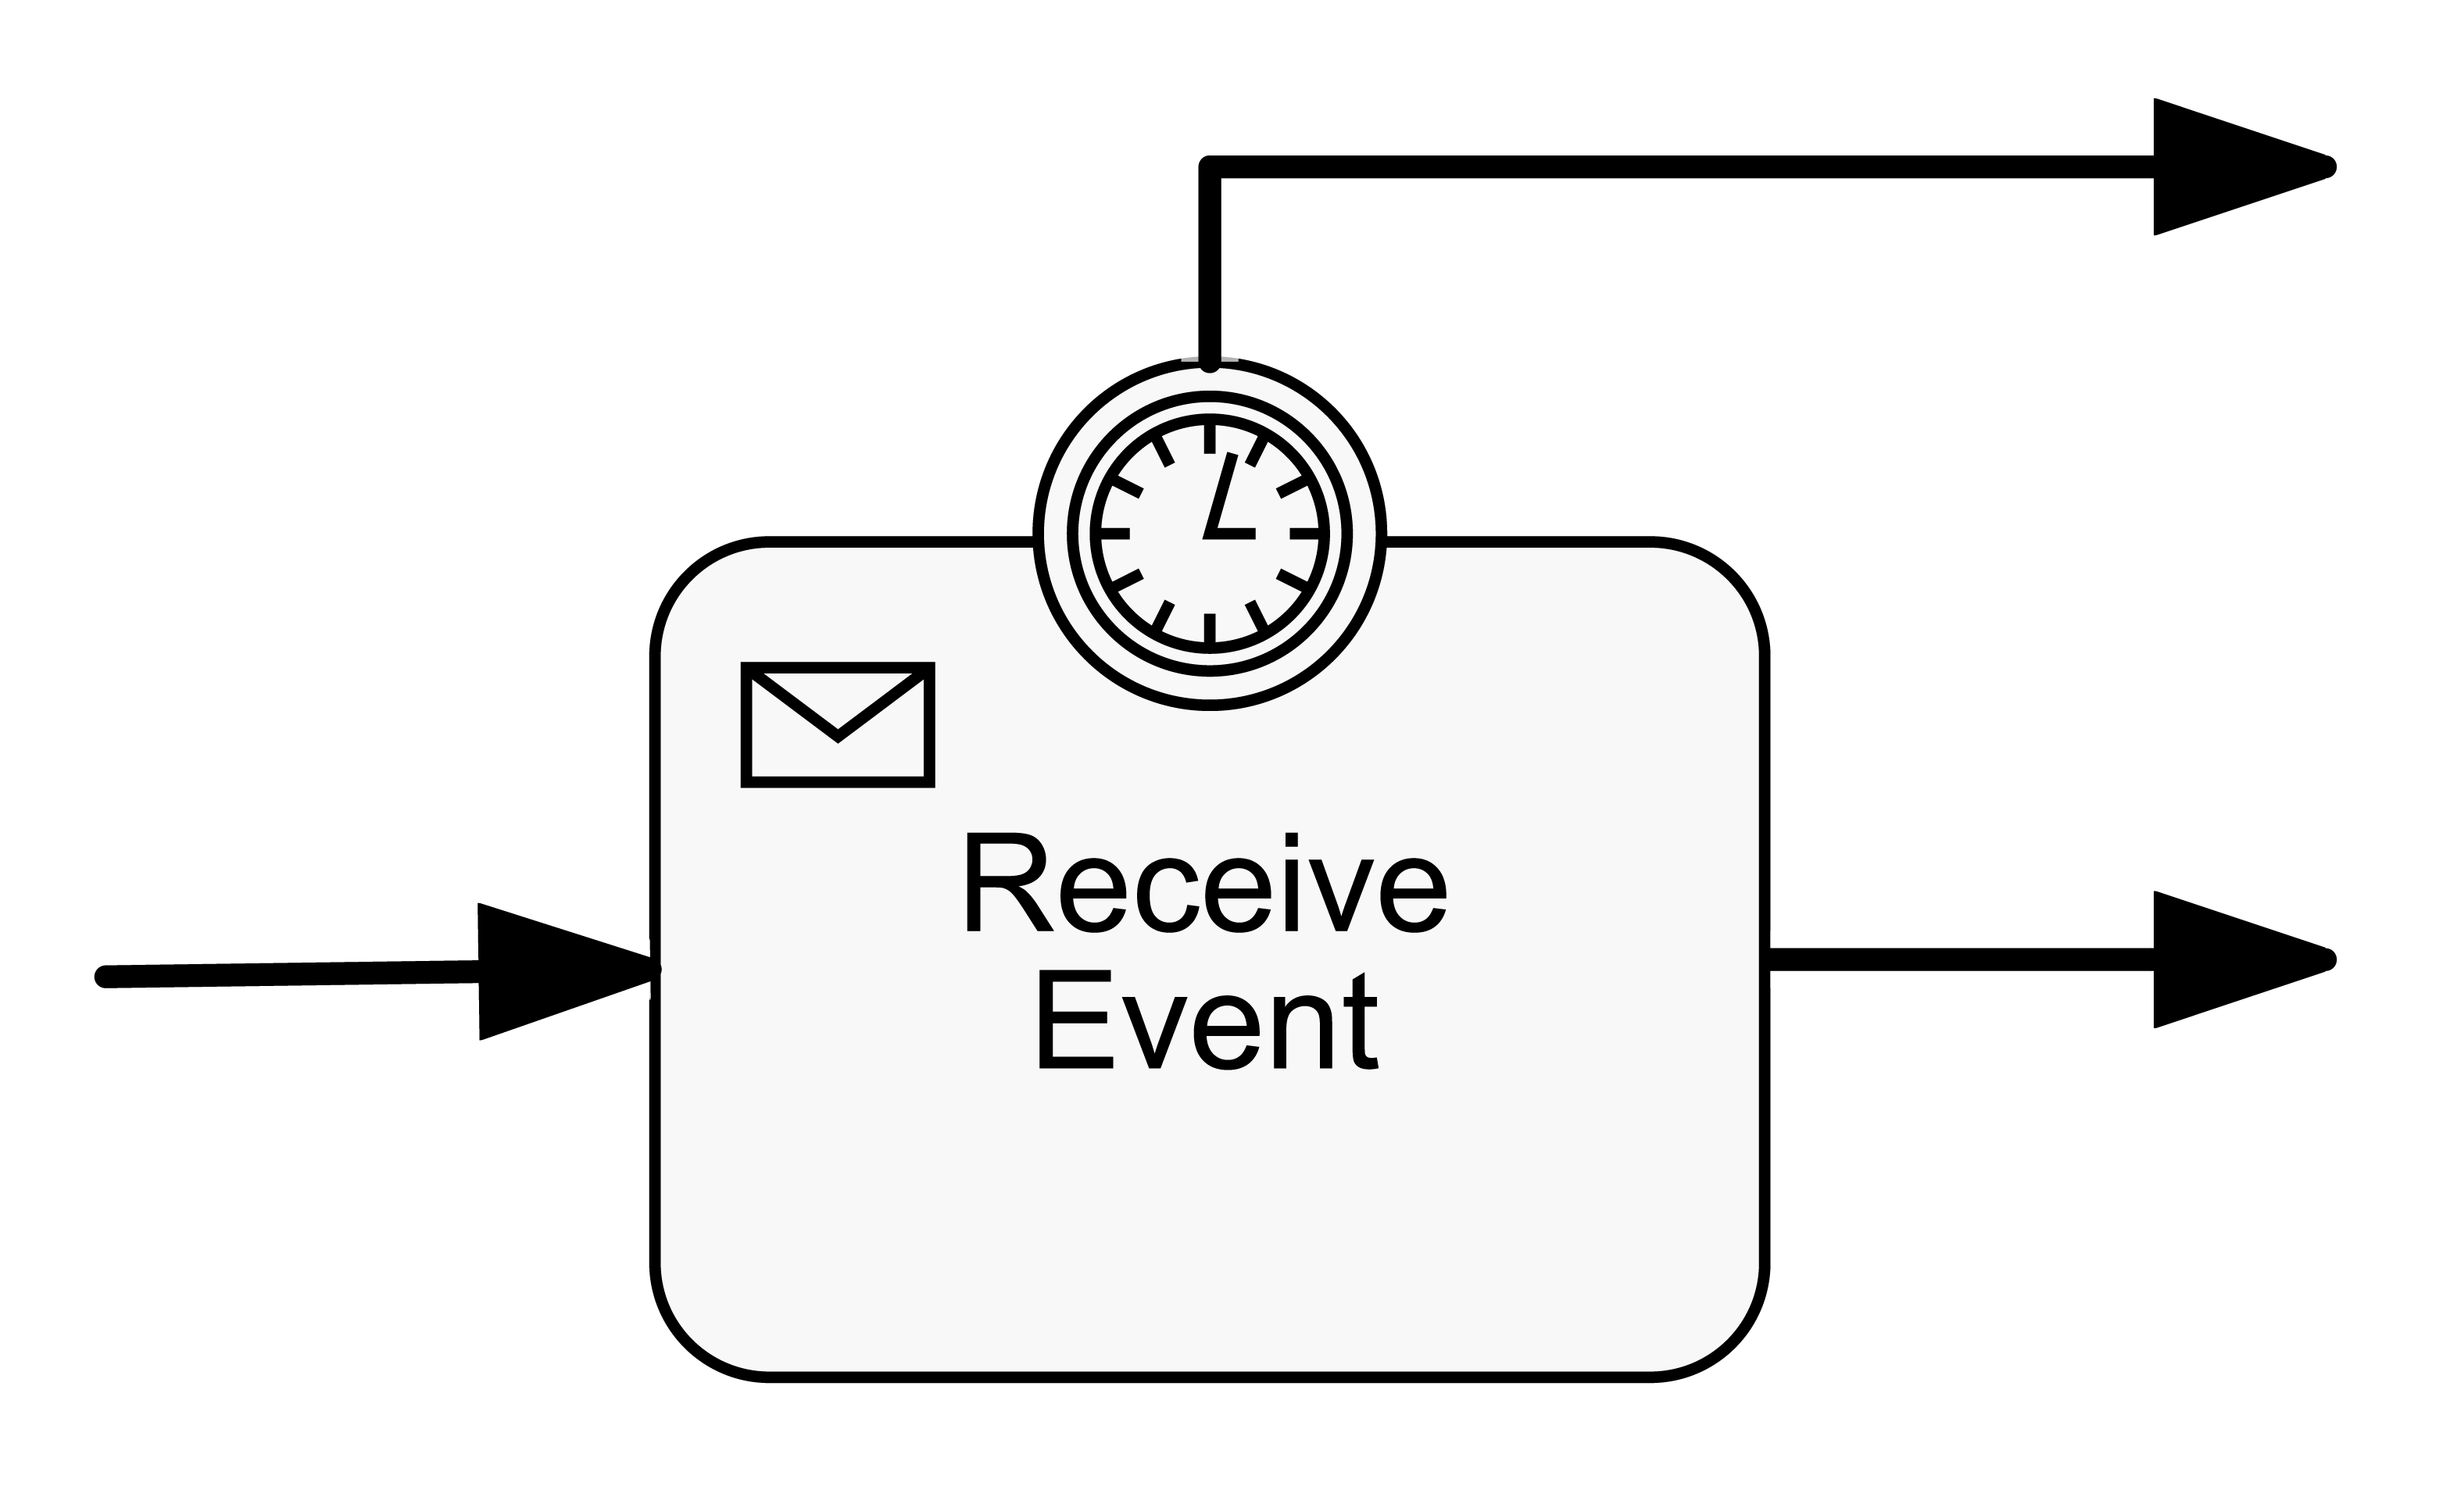
\includegraphics[width=.45\linewidth]{chapters/assessment/boundary-timer-event.png}}
	\caption{Receipt of an intermediate message event, either interrupted by a~boundary event\,(a) or parallel timer event\,(b).}
	\label{fig:excerpt-event-with-timer}
\end{figure}

In certain situations an event might not occur at all. Given a basic event implementation like in \autoref{fig:abstract-process-with-event}, the process flow will get to a halt once it reaches the intermediate catch event and will not be able to proceed. While, depending on the process design, this might be the desired behavior, in many situations this is not acceptable.
In \textit{Example~1.2}, the process relies on the \textit{final arrival time} information from the customer. If the event does not occur, for example due to a mistake in a factory work-flow, the process execution waits for the event indefinitely.
To improve the process design, the logistics company decides that after waiting for the event for 30~minutes, an arbitrary delivery window shall be assumed. The waiting for the event shall be terminated so that the goods can be delivered immediately.

\autoref{fig:excerpt-event-with-timer} shows how this behavior can be implemented in two ways: (a)~By the help of an event-based gateway which puts a timer event in parallel to the intermediate catch event: If the timer event occurs before the message event is consumed, the message event is terminated immediately and the process flow proceeds from the timer event.
An alternative solution with equivalent semantics is depicted in~(b), using a receive task and an interrupting boundary timer event. Once the timer event fires, the receive activity is canceled and the process continues along the outgoing flow of the time event.
Any of the two model improvements will make sure that a process does not run into a lock if the expected event does not occur.


\subsection*{EOS3: Occurrence between Process instantiation and the enabling of the BPMN event}
\begin{figure}[]
	\myfloatalign
	{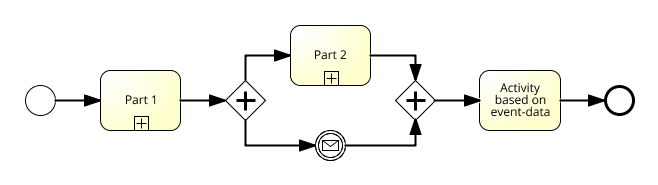
\includegraphics[width=1\linewidth]{chapters/assessment/parallel-gateway-early-subscription.png}}
	\caption{Event Element in parallel process flow}\label{fig:excerpt-parallel-gateway-event}
\end{figure}

In case the event occurs during process execution, but before the BPMN event element is enabled and thus listening for events, the occurrence will not be available for consumption. 
The execution will come to a halt at the event element as if the event did not happen at all.

To avoid a lock in this scenario, the intermediate catch event can be placed in parallel to the rest of the process flow using a parallel gateway. 
This is illustrated in \autoref{fig:excerpt-parallel-gateway-event}. The time of subscription to the event can be controlled by the position of the parallel split: To implement an event subscription right after process instantiation, the Parallel Gateway has to be the first element after the Start Event~(that means \textit{Part~1} in the illustration is empty). 
To implement the event subscription at a specific point during process execution, part of the process must execute before reaching the Parallel Gateway. As modeled in \autoref{fig:excerpt-parallel-gateway-event}, the event may occur at any time during the execution of the collapsed sub-process \textit{Part~2}. 

\subsection*{EOS4 and EOS5: Before Process Instantiation}\label{ass:model:buffered}
\begin{figure}[]
	\myfloatalign
	{\hspace*{-1.0cm}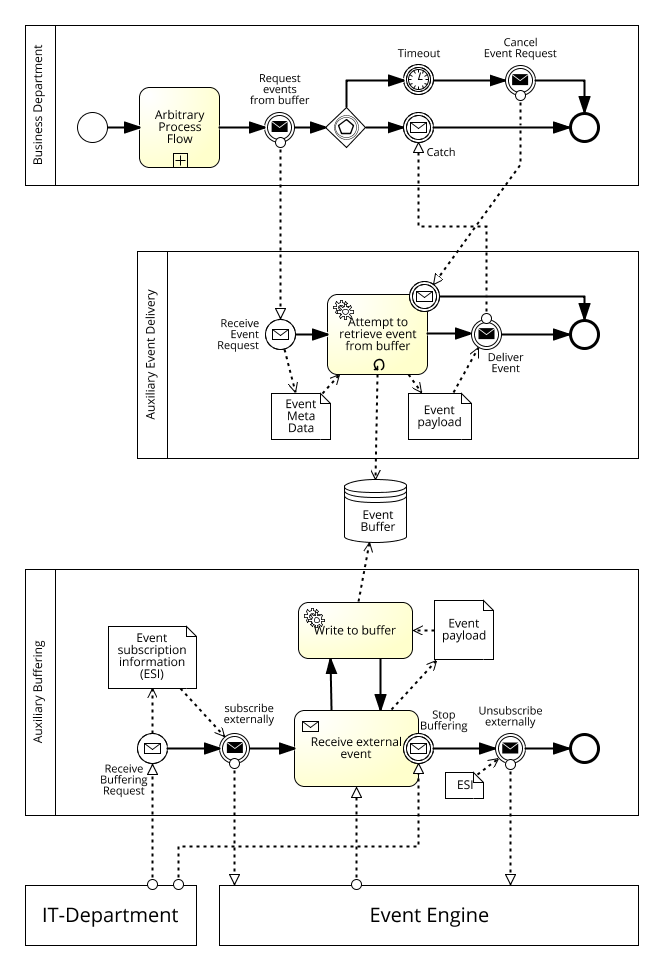
\includegraphics[width=1.2\linewidth]{chapters/assessment/EOS5_buffer_pushing.png}}
	\caption{Event Buffering through an auxiliary buffering process}\label{fig:aux-buffering-process}
\end{figure}

%intro
Any Events that happen before process instantiation will not be considered in a standard intermediate catch event. That applies to both scenarios, the occurrence between deployment and instantiation~(\textit{EOS4}) and an occurrence time before the deployment of the process in the Process Engine~(\textit{EOS5}).

%new elements
To create a process model that allows to catch an event before the process instance exists, three new elements are introduced in addition to the existing process referred to as \textit{target-} or \textit{original process}. The elements are: (1)~An additional \textit{Auxiliary Buffering Process}~(or \textit{buffering process}) that can catch an incoming event independently from the target process; (2)~an \textit{Event~Buffer}, a temporary data-store that keeps event data until it is ready for consumption; (3)~an \textit{Auxiliary Event Delivery Process}~(or \textit{delivery process}), that retrieves events from the buffer and makes them available to the target process.
By introducing an additional process for listening to the event, the subscription time to the \textit{Event Engine} can be before instantiation or even deployment of the original process.
\autoref{fig:aux-buffering-process} shows the interaction of the original process, the two auxiliary processes and the data-store.
\todo[inline]{thus also addressing requirement 3}

%how does that work in detail
%Auxiliary buffering
\paragraph{The execution flow}
To start listening for an event, the auxiliary buffering process has to be instantiated through a message start event containing the information necessary for the event subscription. Considering that the related process instance is not yet running, it is assumed that participants from the \textit{IT-Department} start the buffering any time before process instantiation.
It is also their task to stop the buffering when it not required anymore, for example when the process gets un-deployed.

The buffering process subscribes to the event engine through a throwing event. It then waits for an event to occur in a receive activity \textit{Receive external event} and outputs the received event data to a DataObject. That object is then written to a persistent, global data-store \textit{Event Buffer} by the service task \textit{Write to buffer}. 
The design is able to handle multiple event occurrences, as the execution flow proceeds back to the receiving activity after writing to the buffer.
The implementation of the service task decides about the exact semantics of the buffering and hence about requirement~\textit{R3.3}. For the sake of simplicity, it is assumed that the buffer can hold a maximum of 1~element~(\textit{Size~Policy}) and the service task overwrites that element whenever a new one is available, specifying the retrieval order~(R3.3.4).
An implementation of the \textit{Lifespan Policy} is not provided. 
The consumption behavior~(\textit{R3.3.2}) is defined by the service task of the auxiliary delivery process: After the retrieval of an event from the buffer it remains available.

%original process and event delivery
After the buffering process is running, the original process can be instantiated. 
%In the presented model, its intermediate catch event has been explicitly split into three events to fulfill the publish/subscribe paradigm: An initial send event to request events, a catch event to receive and a final send event to signal that no events shall be received anymore.
After completing the \textit{Arbitrary Process Flow}, a send event instantiates the \textit{Auxiliary Event Delivery Process}, which tries to read from the event buffer and delivers the event to the original process if there is one available. 
The central looping activity will retry reading from the buffer until data becomes available.
In the provided example, the original process will alternatively stop waiting for the message reception as soon as the time event fires. In that case, the delivery process is stopped by an additional message throw event and both processes stop.
Note that the delivery process is designed to retrieve and deliver a single message from the buffer.

%conclusions
\paragraph{Conclusions}
Thanks to the complex interaction of the three processes, the original process can consume the desired event, even though the event occurs before process instantiation. Consequently, \textit{EOS4}~can be handled by the model. 
Moreover, the \textit{Auxiliary Buffering Process} is not bound to a specific event, it works generically with any event information that is passed to it. For that reason it is also not bound to a specific process deployment and can buffer events even before a process has been deployed, so it handles scenario~\textit{EOS5}.
The buffering process can alternatively be started using an explicit message send event during process execution, similar to the \textit{Explicit Subscription Task} introduced in \cite{mandal:2017}. By that means, the event subscription on process instantiation or at any time during process execution is also supported, which results in the fulfillment of requirement~\textit{R2.2}.

%BUT
It remains to be highlighted that this approach will only work for \textit{EOS4} and \textit{EOS5} if the buffering process is instantiated before the associated event occurs. As there are no other systems in place to automatically instantiate the process, it must be assumed that the process is manually started for each event and each process model that requires an early event subscription.
Furthermore, the number of processes running in the execution environment increases significantly. An instance of the buffering process is required for each event element that ought to make use of an event subscription time before deployment. For each instance of the original process and each buffered event, an instance of the auxiliary event delivery process must be started.

\medskip \noindent
More precisely: Given a process $P1$ with a number~$n_{bea}$ of event elements that subscribe after instantiation, and a number~$n_{beb}$ of elements that subscribe before instantiation of $P1$. Furthermore, the buffering process~$BP$ and the delivery process~$DP$, then the number of instances~$instances(P)$ with $P$ being an arbitrary process is as follows:

\begin{itemize}
	\item $instances(BP) = n_{beb} + instances(P) \times n_{bea} $
	\item $instances(DP) = instances(P) \times (n_{beb} + n_{bea})$, assuming that exactly 1 instance of each event is currently in waiting state.
\end{itemize}

\noindent That puts additional load on the process engine which can endanger the reliability of business-critical processes and makes the management of processes and their instances more complex.
The downsides of the presented approaches are discussed in more detail in \autoref{ch:ass:discussion}.


\section{Flexible Event Subscription in standard Camunda}\label{ch:assessment-implementation}
The previous chapter has shown that it is possible to create BPMN models to match each of the Event Occurrence Scenarios, though for the scenarios \textit{EOS4} and \textit{EOS5} the solution becomes increasingly complex.
In the next step I investigate the capabilities of Camunda as an example for a state-of-the-art business process engine.
Camunda shall be used without any code customization, that means as offered through the deployment package.
The solution presented in \autoref{ass:model:buffered} (\textit{EOS4} and \textit{EOS5}) has proven capable enough to handle all event occurrence scenarios, it is therefor the goal to implement a prototypical solution in Camunda in strong accordance with the BPMN model shown in \autoref{fig:aux-buffering-process}.

Two generic sample processes have been modeled for evaluate the functionality of the system. \autoref{fig:camunda-example-o3} shows a simple process with an explicit subscription activity to represent the listening to the event after process instantiation but before reaching the Catch Event (Scenario~\textit{EOS3}). It follows a sample activity that takes 15 seconds (implemented using a \textit{Script~Task}), the intermediate catch event and another script task that displays the content of the received message.
The example for scenarios \textit{EOS4} and \textit{EOS5}~(\autoref{fig:camunda-example-o4-o5}) comprises the following elements: After the start event follows an intermediate catch event, then an activity that prints the message of the event to console and last the process end event. Both figures show screen captures from the Camunda Modeler.

\begin{figure}[]
	\myfloatalign
	{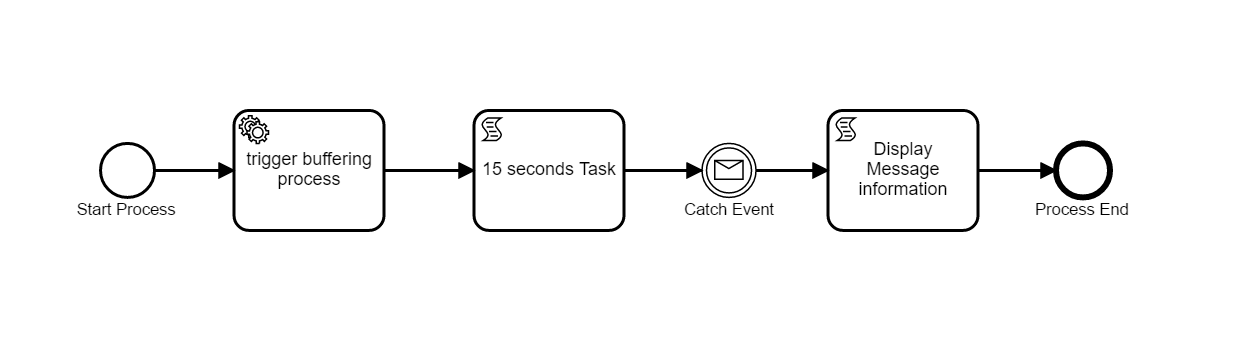
\includegraphics[width=1\linewidth]{chapters/assessment/example-o3.PNG}}
	\caption{Generic Example Process in Camunda for \textit{EOS3}}\label{fig:camunda-example-o3}
\end{figure}

\begin{figure}[]
	\myfloatalign
	{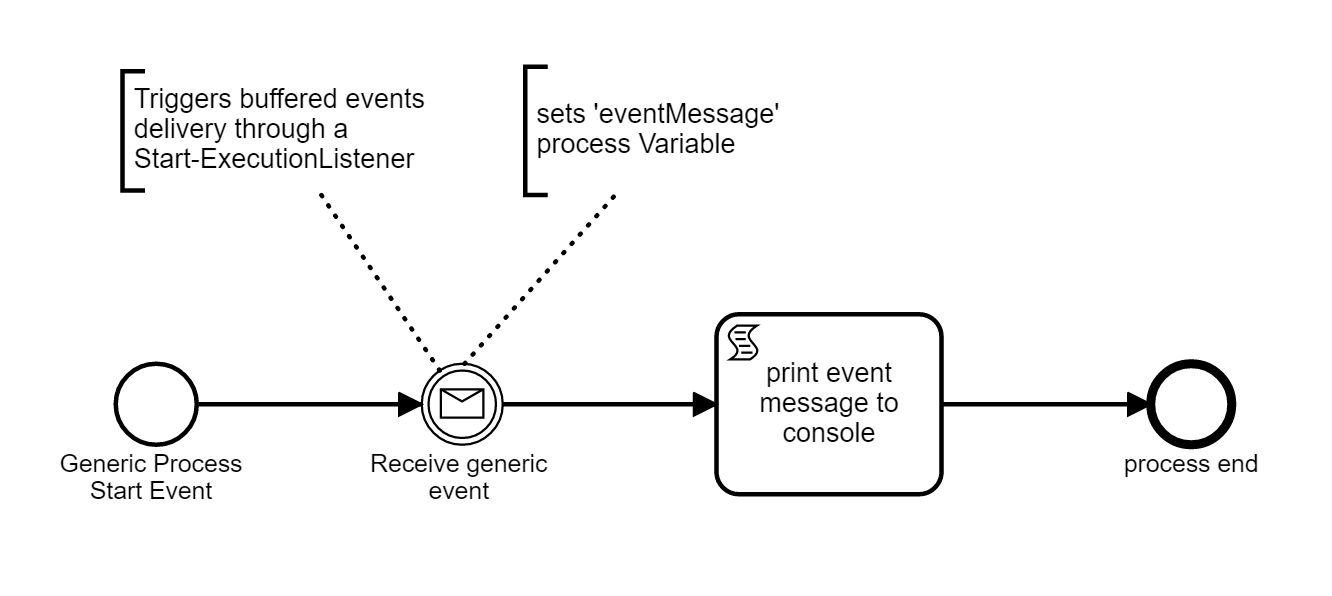
\includegraphics[width=1\linewidth]{chapters/assessment/example-o4-o5.PNG}}
	\caption{Generic Example Process in Camunda for the Event Occurrence Scenarios \textit{EOS4} and \textit{EOS5}}\label{fig:camunda-example-o4-o5}
\end{figure}

\paragraph{Auxiliary Buffering Process}
The task of this process is to subscribe to a CEP Platform using a provided event query and start listening for events. Any incoming event must be stored in a data-store (\textit{Event Buffer}).
A local MySQL database has been chosen for persisting the event data because it is freely available, easy to set up, offers standardized access via SQL queries and Java connectors.
As complex event processing functionality itself is not required to demonstrate the use-case, the role of the \textit{Event Engine} is taken by a basic web-service which was specifically implemented in Python. It exposes a \textit{subscribe} method via \acs{HTTP} and can be used to trigger event messages associated to registered subscriptions.

\autoref{fig:camunda-aux-buffering-process} shows the final Buffering Process modeled in the Camunda Process Modeler. The process can be instantiated by issuing a \textit{Buffering Task} message. This message must contain three data fields: \textit{processDefinitionId}, to know which process definition the buffered messages belong to; \textit{messageName}, the name of the message event within the process; \textit{query}, the event query in the Esper Query Language.
Camunda will make the message data automatically available in the process instance as process variables, so they can be used during the execution of the Buffering Process.
After instantiation, the process reaches the activity \textit{Subscribe to Event Source}, a \textit{Java Service Task} that executes a HTTP call to the event engine. That call registers the event query in the platform, providing the process instance identifier and the message name. Based on this information, Camunda can correlate received events back to a specific process instance and message element.
After the subscription, the process reaches the receiving activity \textit{Wait for unsubscribe event} that will terminate the process as soon as the \textit{Unsubscribe} event has been received.
As long as this activity is active, events can be received through the attached non-interrupting boundary event. Incoming events have a field \textit{eventBody}, which contains the event information and becomes available through a process variable with the same name.
The boundary event triggers the service task \textit{Write eventBody to datastore}, which takes the data from the process variable and writes it to the MySQL Database (\textit{Global Event Buffer}).

%Notably, the Camunda process model appears less complex than the one presented in \autoref{ass:model:buffered} while still implementing the same functionality.

\begin{figure}[]
	\myfloatalign
	{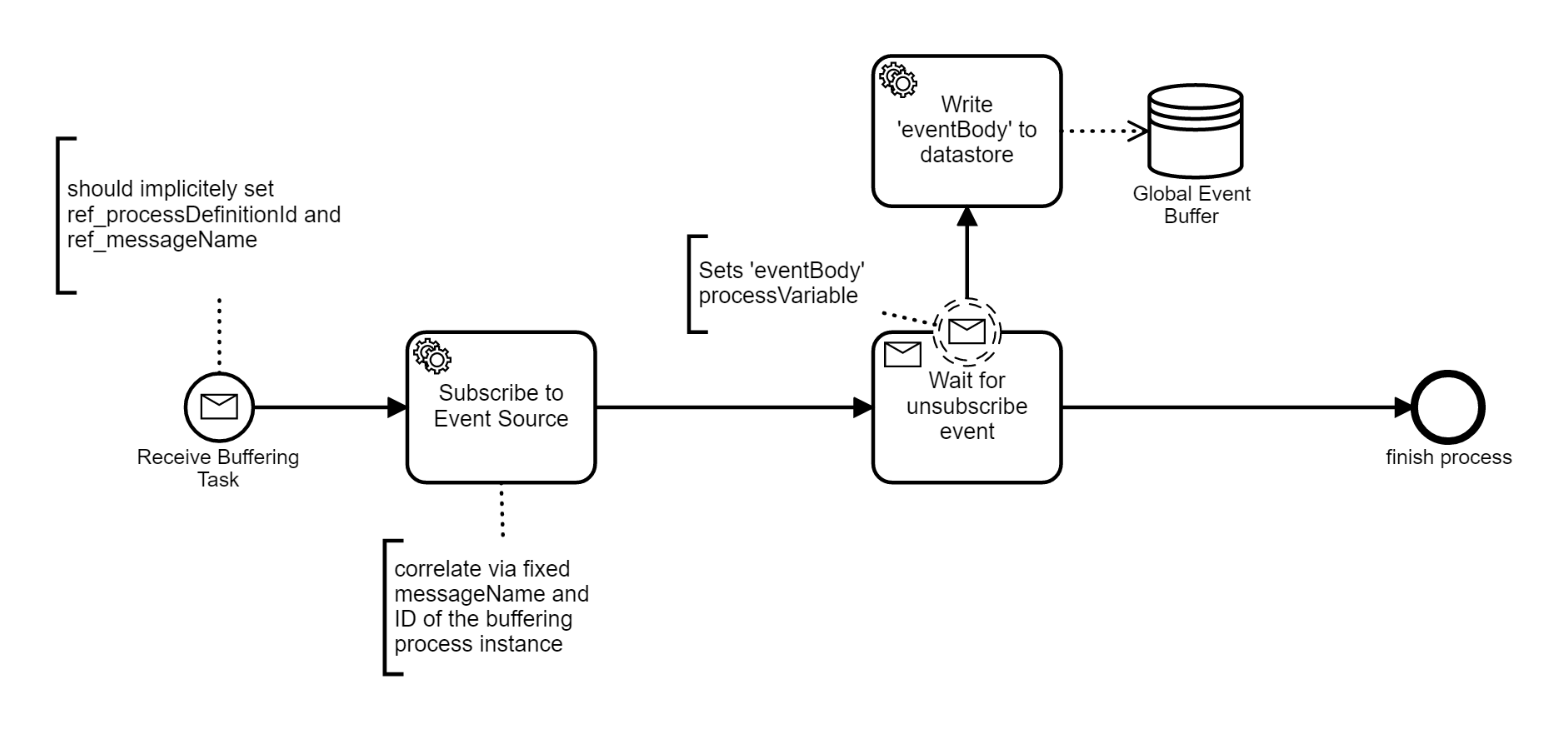
\includegraphics[width=1\linewidth]{chapters/assessment/buffering-process.PNG}}
	\caption{Auxiliary Buffering Process in the Camunda Modeler}\label{fig:camunda-aux-buffering-process}
\end{figure}

\paragraph{Auxiliary Event Delivery Process}
The delivery process (see \autoref{fig:camunda-aux-event-delivery}) reads the latest data from the buffer and sends it to the process instance. It can be started with a message that contains the \textit{processInstanceId} and the \textit{processDefinitionId} of the requesting process and the \textit{messageName} of the message event that is requested from the buffer.
A timer event \textit{Delay Timer} has been inserted to make sure that the requesting process is already listening for an event, when the delivery process sends the message. The outgoing execution flow is treated asynchronously.
It follows the service task \textit{Retrieve event from buffer}, which executes Java code to read from the MySQL Database \textit{Event Buffer} and store the event information in a process variable named \textit{eventMessage}.
The content of that process variable is sent to the original process in the send event, afterwards the execution is finished.

\begin{figure}[]
	\myfloatalign
	{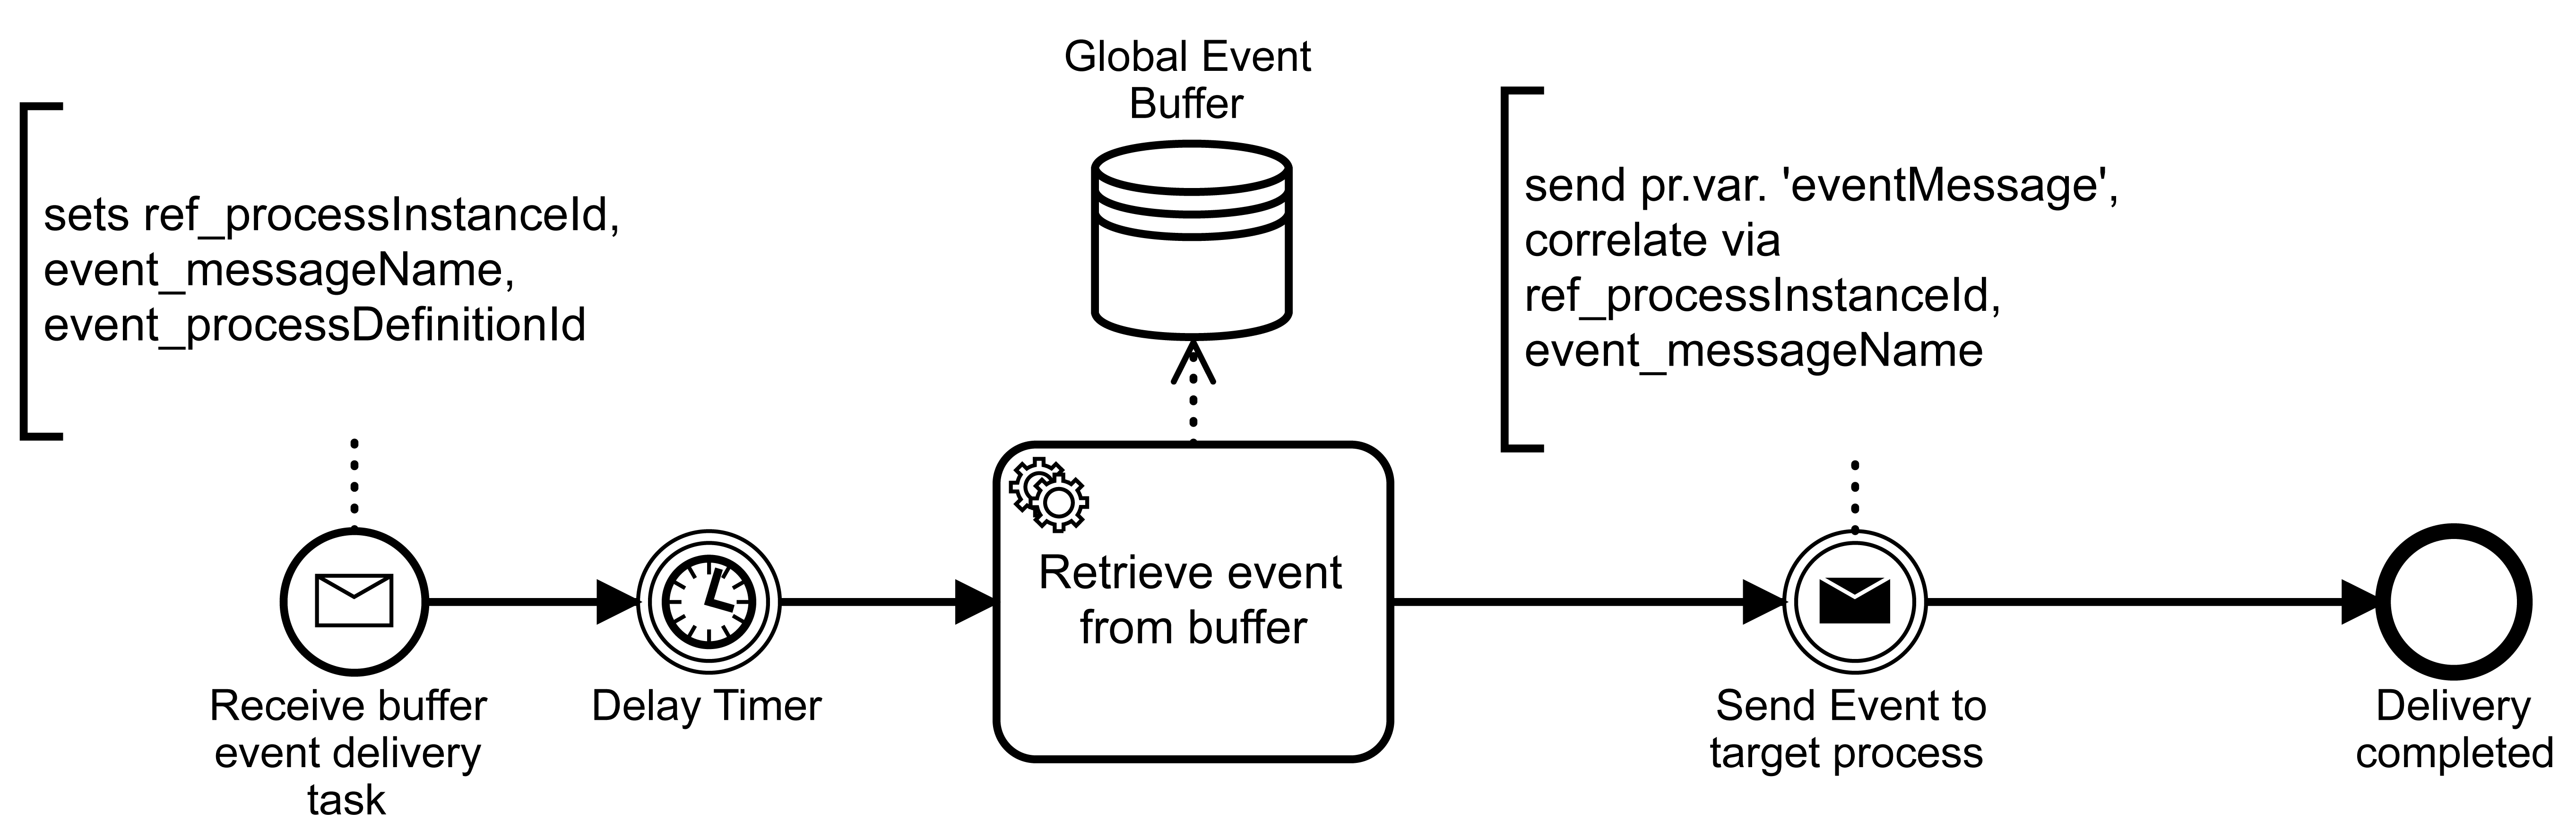
\includegraphics[width=1\linewidth]{chapters/assessment/buffer-delivery-process.PNG}}
	\caption{Auxiliary Event Delivery Process in Camunda Modeler}\label{fig:camunda-aux-event-delivery}
\end{figure}


\paragraph{Interaction of the Processes}
%In this implementation of flexible event subscription, the action of subscribing to the event source and the reception of events in the Original Process are splitted into two separate parts, each supported by an auxiliary process.
To initiate the subscription at the event source, the Auxiliary Event Buffering process has to be started.
For scenario \textit{EOS3}, this happens through an extra activity (\textit{Trigger Buffering Process}) during process execution, so that events after process instantiation are received by the Buffering Process.
In scenarios \textit{EOS4} and \textit{EOS5}, the subscription and thus the instantiation of the Buffering Process must happen before the instantiation of the Target Process. As there is no such mechanism in the standard Camunda Process Engine, the Buffering Process must be started manually, providing the \textit{processDefinitionId}, the \textit{messageName} and the \textit{eventQuery}.

Now that the \textit{Buffering Process} is running, any events matching the query will be stored to the buffer.
When the Target Process reaches the Catch Event, a request for buffered events is sent as a message to trigger the \textit{Auxiliary Event Delivery Process}.
This message is sent using a short piece of Java code that gets executed when the Catch Event is reached. 
The code is invoked by a Start ExecutionListener attached to the Catch Event. ExecutionListeners are offered by Camunda to execute own Java programs before or after relevant events during process execution, like the execution of an element in the process.
While the Original Process will now start listening for the desired events, the Event Delivery Process will send the buffered events as messages to the Original Process.

If no events have been received yet, all the involved processes remain active: the Buffering Process will keep listening for an external event. The Delivery Process will send an event to the Original Process as soon as there is one in the buffer. The Catch Event in the Original Process will keep listening for an Event.
The necessary communication for the termination of the processes and the unsubscribe-operation have not been implemented in this prototypical implementation, as they would not add particular value to the evaluation.

The code of the Camunda process application is provided as part of the deliverables of this thesis.


\paragraph{Conclusion}
The described implementation of the BPMN buffering concept presented in \autoref{ass:model:buffered} serves as a brief evaluation of the model. As illustrated by the help of the two examples, the resulting set of process applications allows to issue an event subscription flexibly according to the event occurrence scenarios.
While a thorough analysis was not the target of this section, it still provides an introduction to the capabilities of the Camunda process engine, which will take an important role again in \ref{ch:implementation}.


Note that this is an investigative implementation that matches exactly the given use-case and is not meant to be used in production. It is neither flexible nor robust enough for that purpose, but suits very well in understanding the capabilities and the shortcomings of BPMN and Camunda when it comes to handling the Event Occurrence Scenarios.

\section{Overview \& Discussion}\label{ch:ass:discussion}
It was the goal of this chapter to evaluate the capabilities of current \acs{BPM} solutions against the requirements presented in \autoref{ch:requirements}.
The evaluation was performed at the example of the \acs{BPMN} without allowing the use of the in-built extension mechanism. Furthermore, the developed BPMN solution for buffered event handling~(\autoref{ass:model:buffered}) was implemented prototypically in Camunda to evaluate the applicability of the concept to a business process engine. % which provides an additional understanding 

Thanks to the flexibility of the BPMN standard, all of the requirements could be expressed in a model, but the solutions significantly vary in complexity.
\autoref{tab:assessment-bpmn} summarizes the results, categorizing the findings into three classes: 
\textit{(+)}~means that the requirement is fulfilled natively and without the necessity for additional elements int the model; 
\textit{(o)}~signifies that there are acceptable ways to express the desired behavior, but additional elements are necessary for that purpose which increases model complexity; 
if the aspect is marked as \textit{(-)}, the solution requires a drastic increase of complexity, which might not be acceptable.
The categorization is based on the findings of the previous sections and a brief explanation is provided in the last column.

%this is all subjective
%note that no aspect could NOT be implemented

\begin{table}%[h]
	\myfloatalign
	\begin{tabularx}{\textwidth}{p{0.3\linewidth} | c | p{0.555\linewidth}}
		\toprule
		\tableheadline{Requirement} & \tableheadline{Ev.} & \tableheadline{Explanation} \\ 
		\midrule
		
		\multicolumn{3}{p{\linewidth}}{\rule{0pt}{4ex} R1: Subscription Fundamentals} \\
		\midrule
		
		R1.1 and R1.2\newline(Un-)\,Subscription to/from the Event Source & o & requires additional model elements, \eg~throw/catch event, send/receive task, service task \\
		R1.3 Availability of Information & o & possible by using Annotation or DataObject  \\
		R1.4 Variables in Event Queries & o & supported through custom implementation in service task \\
		
		\midrule
		\multicolumn{3}{p{\linewidth}}{\rule{0pt}{4ex} R2: Event Subscription Time} \\
		\midrule
		
		R2.1 Explicitness & o & not explicitly stated by BPMN, but possible to derive \\
		R2.2 Flexibility & & \\
		> EOS1 & + & natively supported \\
		> EOS2, EOS3 & o & added complexity through parallel process flow \\
		> EOS4, EOS5 & - & requires auxiliary processes, significant increase of model elements \\
		R2.3 Awareness of Subscription Dependencies & o & if subscription is modeled explicitly, a DataInput can be used \\
		
		\midrule
		\multicolumn{3}{p{\linewidth}}{\rule{0pt}{4ex} R3: Event Buffering} \\
		\midrule
		
		R3.1 Buffering Principle & + & Temporary storage can be expressed through DataObjects \\
		R3.2 Buffer Scope & o & DataObjects for instance-scope, DataStore otherwise. Interaction with data-store adds complexity. \\
		R3.3 Buffer Policies & o & by textual description or the implementation-specifics of a service task; pure graphical representation will become extremely complex. \\
			%Note that complex policies like the retrieval order, buffer size and consumption behavior can theoretically be expressed in a BPMN graph, but become exponentially complex.} 
		
		%\bottomrule
	\end{tabularx}
	\caption[]{Overview of the assessment of BPMN against the requirements}
	\label{tab:assessment-bpmn}
\end{table}

\medskip \noindent
As revealed in the tabular overview, a means to express the required behavior could be found for each of the aspects.
However, only two of them are considered to be natively supported by the standard while most of the concepts reveal certain shortcomings when it comes to modeling flexible event subscription using BPMN. 
%requirements add additional complexity to the solution. %specific work-arounds had to be identified.
In the following, the identified shortcomings are discussed one after the other. The discussion is arranged into three parts which are specifically marked as \textit{S1} to \textit{S3}. The shortcomings should be specifically addressed in addition to the requirements \textit{R1} to \textit{R3} when developing solutions to flexible event subscription.

%- a model of buffered event handling and event subscription in bpmn has been presented and successfully implemented in Camunda.

\subsection*{Shortcoming S1: The necessary additional process elements increase model complexity and hence reduce comprehensibility.}

The topic of model complexity has been investigated for example by Mendling~et.\,al.\,\cite{mendling2008metrics,mendling2010seven} and Vanderfeesten~et.\,al.\,\cite{vf2007quality}.
In their work on process modeling guidelines\,\cite{mendling2010seven}, Mendling~et.\,al. state that \textit{without a proper understanding of the business process [...] they are doomed to fail)}.
One of the main reasons for decreased comprehensibility lies in the amount of elements and routing paths.

\subsubsection*{S1.1: Additional process elements are required within the additional process.}

Most of the presented approaches require additional process elements or even entire processes to implement the behavior.
To cope with the event occurrence scenarios \textit{EOS2} and \textit{EOS3}, the introduction of additional gateways and therefor routing paths is necessary for each event element that is supposed to use flexible event subscription.
Due to that dependency on the number of buffered events in the process, the added complexity will increase linearly with that number.

\subsubsection*{S1.2: Two more participants must be added to implement the subscription before instantiation.}

Another dimension becomes apparent in the BPMN model for buffered event handling that is presented at the end of \autoref{ass:model:buffered}. While it allows the subscription to events even before process deployment, it requires the execution of an additional set of auxiliary processes for that purpose.
Consequently, the increase of process elements is accompanied by an increase of participants. A simple model involving only one event will blow up into a complex process model with three pools, being less concentrated on the actual business case.

The increased complexity will not only make the resulting model more difficult to understand, but also complicate the design phase by requiring a basic understanding of the publish/subscribe model, the usage semantics of the auxiliary processes and the patterns revealed to control subscription time within a process instance.

%how to create process models that analysts and business professionals can easily analyze and understand. 

\subsection*{Shortcoming S2: Event buffering and subscription are infrastructure tasks and therefor not suited to be implemented through a business process model.}
Arguably, the buffering of data and the subscription and un-subscription from events are not business tasks and should hence not be entirely modeled in a business process.

\subsubsection*{S2.1: The buffering and subscription activities pollute the model with non-business-related content.}
Though necessary to allow the successful execution of the process, the effort to enable flexible event subscription stands in no relation to the business value it represents. The models essentially get polluted with non-business-related process segments.
It can be observed from the findings of this chapter, that it is not handy to model the required functionality in the BPMN. After all, two essential activities within the auxiliary tasks are still service tasks. Although the notation allows these kind of code-based tasks, their detailed behavior is still hidden within the underlying implementation.

\subsubsection*{S2.2: Process designers likely lack the skills to cope with event buffering and subscription.}
Moreover, as noted in \textit{S1}, the design of a process gets more complicated due to the increased number of elements.
Another issue to consider in that matter is that the process designer who has to make use of the auxiliary processes usually does not have a comprehensive knowledge in information technology~(see~\cite{weske:bpm-book},\,p.\,16). An additional stakeholder will have to be included in the design process, resulting in more complex workflows.

Once a given process has been deployed in a process engine, it has to be monitored and maintained.
Given that even the simplest process involves the execution of two additional instances for buffering, any maintenance and search for errors will be significantly more complicated.
Just like in the design phase, the maintenance will require knowledge of event subscription and buffering, which is probably not available by default.


\subsection*{Shortcoming S3: Implementing event buffering through process models is likely to cause performance issues.}

\subsubsection*{S3.1: The execution of additional buffering processes affects process engine reliability.}

%buffering slows down execution of business-critical processes, makes less reliable
Because of the buffering and delivery jobs, two additional processes are potentially running in parallel to any given process instance. For each Event Element used in a process, the engine has to execute an instance of the buffering process and, eventually, an instance of the buffer delivery process.
For example in a process using two event elements, one subscribing at deployment time and one subscribing after event instantiation, \textbf{the maximum number of process instances for a single execution increases from~1~to~5}. An exact formula to determine the number of instances is provided in \ref{ass:model:buffered}.


It is not only the increase in the number of processes, but also the kind of work the the processes are executing: Each instance of the auxiliary buffering process constantly listens to an event source, potentially receiving events and thus creating load in sub-second scale.
Instead of only listening to an event source when the event element is reached, the process engine has to listen, receive, process and write to the buffer all the time. Even if no instance of the original process is about to use the events.
That increase of running process instances puts additional load on the process engine, which might prevent business critical processes from executing without delays. 
Taking into consideration that a process engine can only handle a limited number of process instances and operations, there is an increased possibility of complete engine failure.

\subsubsection*{S3.2: The execution of event buffering through a business process is limited by process engine performance.}
	
%process execution engine too slow for buffering
Apart from the reduced reliability and the possible delay to the execution of the processes, there is a second performance-related perspective to the issue.
Given the large amount and high frequency in that events can occur in reality, optimal performance is required for an event-buffering module. 
Depending on the event query and frequency of event occurrence, the engine has to be ready to receive events at a very fast pace.
When executing these operations from a BPMN model inside a process engine, the speed in that steps can be executed is only as fast as the process engine itself. While complex event processing platforms are optimized to handle many events in a short amount of time, a process engine is not built for that purpose and might fail to deliver the required performance.
An aspect that cannot be influenced without customizing the process engine code.

% there remains an event-management overhead as every event has to be handled twice: once when it is stored in the buffer and once when it's delivered to the target process.

%\paragraph{Hidden Performance Limitations of the Process Engine\newline}
%The buffering process and the delivery process are designed to be generic so that only two more process definitions need to be available in the process repository.
%The number of process instances instead will greatly increase 


